

\title[概率论]{第六讲:条件概率、全概率公式与贝叶斯公式}
%\author[张鑫 {\rm Email: xzhangseu@seu.edu.cn} ]{\large 张 鑫}
\institute[东南大学数学学院]{\large \textrm{Email: xzhangseu@seu.edu.cn} \\ \quad  \\
	\large 东南大学 \quad 数学学院 \\
	\vspace{0.3cm}
	%\trc{公共邮箱: \textrm{zy.prob@qq.com}\\
		% \hspace{-1.7cm}  密 \qquad 码: \textrm{seu!prob}}
}
\date{}


{\setbeamertemplate{footline}{}
	\begin{frame}
		\titlepage
	\end{frame}
}


%\subsection{条件概率}
%\begin{frame}{条件概率的引入}
%	\begin{itemize}
%		\item 有时除了 $P (\Omega)=1$ 的总前提之外,还会出现附加前提
%		\item 例如,抛掷一枚均匀的骰子一次,已知掷出的点数为奇数,要求求出点数大于 $1$ 的概率,那么此时 “已知掷出的点数为奇数” 就是一个附加前提
%		\item 有附加前提时的概率 $\Rightarrow$ 条件概率
%	\end{itemize}
%\end{frame}
\subsection{条件思考的重要性}%%%%%%%%%%%%%%%%%%%%%%%%%%%%%%%%%%%%%%%%%%%

\begin{frame}{条件思考的重要性}
	\begin{itemize}[<+-|alert@+>]
		\item 条件概率说明了如何以合乎逻辑且相一致的方式将证据纳入人们对世界的理解当中.
        \item 添加条件是一种非常有用的解决问题的策略.
        \item 条件既可以作为更新判断依据的方法,也是解决问题的策略.
        \item 条件是统计学的灵魂.
	\end{itemize}

\end{frame}

\subsection{条件概率的定义和直观解释}%%%%%%%%%%%%%%%%%%%%%%%%%%%%%%%
\begin{frame}{条件概率的引入}
	\begin{exam}
		抛掷一枚均匀的骰子一次,已知掷出的点数为奇数,试求点数大于$1$的概率。
	\end{exam}
	\pause

	\vspace{0.2cm}

		\begin{itemize}[<+-|alert@+>]
			\item $\Omega=\{1,2,\cdots,6\}, A=\{1,3,5\}, B=\{2,3,4,5,6\}$;
			\item 令$P(B|A)$表示“已知$A$发生的情况下$B$发生的概率”;%$\Rightarrow$ 记作
			\item $A=\{1,3,5\}$, \pause $B$发生就是$AB=\{3,5\}$发生,于是
			$$P(B|A)=\frac{|AB|}{|A|}=\frac{2}{3}.$$\pause
			\item 在原样本空间考虑:
			$$P(AB)=\frac{|AB|}{|\Omega|}=\frac{2}{6},\quad P(A)=\frac{|A|}{|\Omega|}=\frac{3}{6}.$$
			\item 易验证:$$P(B|A)=\frac{P(AB)}{P(A)}=\frac{2}{3}.$$
		\end{itemize}

\end{frame}

\begin{frame}{条件概率的引入}
	\begin{exam}
		从分别写有号码$1,2,\cdots,10$的$10$张卡片中随机抽取一张,已知抽出的卡片的号码不小于$3$,试求其号码为偶数的概率。
	\end{exam}
	\pause
	\vspace{0.2cm}

		\begin{itemize}[<+-|alert@+>]
			\item $\Omega=\{1,2,\cdots,10\}, A=\{3,4,\cdots,10\}, B=\{2,4,6,8,10\}$;
			\item 类似上一例:
			$$P(B|A)=\frac{|AB|}{|A|}=\frac{4}{8}=\frac{1}{2}.$$
			\item 在原样本空间考虑:
			$$P(AB)=\frac{|AB|}{|\Omega|}=\frac{4}{10}=\frac{2}{5},\quad P(A)=\frac{|A|}{|\Omega|}=\frac{8}{10}=\frac{4}{5}.$$
			\item 易验证:$$P(B|A)=\frac{P(AB)}{P(A)}=\frac{1}{2}.$$
		\end{itemize}

\end{frame}

\begin{frame}
	\frametitle{条件概率的引入}
	\begin{exam}
		考察有两个小孩的家庭,其样本空间为$\Omega:=\{bb,bg,gb,gg\}$,其中$b, g$分别表男孩与女孩,$bg$表示大的是男孩,小的是女孩,其他样本点类似说明. 在$\Omega$中的四个样本点可能情况下,我们讨论如下事件的概率:
		\vspace{0.2cm}
		\begin{itemize}[<+-|alert@+>]
			\item 事件$A:=\{\mbox{家中至少有一个女孩}\}$发生的概率为$P(A)=\dfrac{3}{4}$
			\item 若已知$B:=\{\mbox{家中至少有一个男孩}\}$发生,再求$A$发生的概率为
			\begin{eqnarray*}
				P(A|B)=\frac{2}{3}
			\end{eqnarray*}
			\item 若对上述条件概率的分子分母各除以4,则有
			\begin{eqnarray*}
				P(A|B)=\frac{2/4}{3/4}=\frac{P(AB)}{P(B)}
			\end{eqnarray*}
		\end{itemize}
	\end{exam}

	\end{frame}

\begin{frame}{条件概率的定义}
	\begin{defi}
		设 $(\Omega,\mathcal{F},P)$ 为概率空间. $A\in\mathcal{F}$, $B\in\mathcal{F}$, 若 $P (B)>0$, 则称 $$P (A|B)=\frac{P (AB)}{P (B)}$$ 为 ``在已知 $B$ 发生的情况下,$A$ 发生的 \textcolor{red}{条件概率}", 简称条件概率.
	\end{defi}
	\pause
	\vspace{0.4cm}
	\begin{rmk} 条件概率的两种计算方法:
		\begin{itemize}[<+-|alert@+>]
			\item 原则性方法: $P (A|B)=\dfrac{P (AB)}{P (B)}$
			\item 把 $B$ 作为样本空间看待 (经常显得非常方便): $P (A|B)=\dfrac{|AB|}{|B|}$
		\end{itemize}
	\end{rmk}
\end{frame}


\begin{frame}{条件概率的例子}
	\begin{exam}
		(两张牌) 洗好一副标准扑克后。从中随机抽取两张牌,无放回地一次抽一张。设 $A$ 事件表示第一张牌为红桃,事件 $B$ 表示第二张牌为红色。求 $P ( A | B )$ 和 $P ( B | A )$.
	\end{exam}

	\begin{jieda}
	  由题意易知
	  \begin{align*}
		P(A\cap B) &=\frac{13 \cdot 25}{52 \cdot 51}=\frac{25}{204}\pause \\
		P(B)&=\frac{26 \cdot 51}{52 \cdot 51}=\frac{1}{2} \\
		P(A) &=\frac{1}{4}
	  \end{align*}
	  \pause
	  从而,
	  \begin{align*}
		P(A|B) &=\frac{P(A\cap B)}{P(B)}=\frac{25/204}{1/2}=\frac{25}{102}\\
		P(B|A) &=\frac{P(B \cap A)}{P(B)}=\frac{25/204}{1/4}=\frac{25}{51}
	  \end{align*}



	\end{jieda}

	\end{frame}
	\begin{frame}{条件概率的注}
	\begin{itemize}[<+-|alert@+>]
	\item 条件概率大小与原事件无条件概率并没有明确的大小关系,见教材例6.5.
	\item  注意哪些事件放在竖线的哪一边是非常重要的,具体来说就是 $P (A|B)\neq P (B|A)$.
	\item 无论 $P (A|B)$ 还是 $P (B|A)$ 都是有意义的 (直观上或数学上):
	\begin{itemize}[<+-|alert@+>]
	   \item 牌抽取的时间顺序并不能决定出现何种条件概率.
	   \item 在计算条件概率时,我们考虑的是一个事件给另一个事件带来的信息,而不是一个事件是否导致了另一个事件.
	\end{itemize}

	\item  此外,也可以通过条件概率的直接解释得出 $P (B|A)=25/51$:
	\begin{itemize}[<+-|alert@+>]
		\item 如果第一张抽的牌为红桃,那么剩下的牌就由 25 张红色牌和 26 张黑色牌组成 (所有牌被下一次抽中的可能性是相同的)
		\item 所以抽取一张红牌的条件概率是 $25/(25+26)=25/51$.
	\end{itemize}
	\end{itemize}

	\end{frame}








\begin{frame}
	\frametitle{条件概率的性质}
	\begin{thm}
		条件概率是概率,即若设 $P(B)>0$, 则
		\begin{itemize}[<+-|alert@+>]
			\item 非负性: $P (A|B)\geq 0, \forall A\in\mathcal{F}$;
			\item 规范性: $P (\Omega|B)=1$;
			\item 可列可加性:若 $A_n\in \mathcal{F}, n=1,2,\cdots,$ 互不相容,则
			\begin{eqnarray*}
				P(\cup_{n=1}^\infty A_n|B)=\sum_{n=1}^\infty P(A_n|B)
			\end{eqnarray*}

		\end{itemize}
	\end{thm}

	\pause \zheng 由条件概率的定义易证非负性与规范性。下面说明可列可加性。假设 $A_n,n=1,\cdots,$ 互不相容,则 $A_nB, n=1,\cdots,$ 也互不相容。从而
	\begin{eqnarray*}
		P(\cup_{n=1}^\infty A_n|B)&=&\frac{P((\cup_{n=1}^\infty A_n)B)}{P(B)}=\frac{P(\cup_{n=1}^\infty (A_nB))}{P(B)}\\
		&=&\sum_{n=1}^\infty \frac{P(A_nB)}{P(B)}=\sum_{n=1}^\infty P(A_n|B).
	\end{eqnarray*}
\end{frame}


\begin{frame}
	\frametitle{乘法公式}
	\begin{thm}[乘法公式]
		\begin{itemize}[<+-|alert@+>]
			\item 若 $P (A)>0$, 则 %\vspace{-0.85cm}
			\begin{eqnarray}
				\label{eq:multiformtwo}
				P(AB)=P(A)P(B|A)
			\end{eqnarray}
			\item 若 $P (A_1A_2\cdots A_{n-1})>0$, 则
			\begin{eqnarray}
				\label{eq:multiformmul}
				P(A_1A_2\cdots A_n)=P(A_1)P(A_2|A_1)P(A_3|A_1A_2)\cdots P(A_n|A_1A_2\cdots A_{n-1})
			\end{eqnarray}

		\end{itemize}
	\end{thm}
	\pause \zheng  由条件概率的定义,移项即得 \eqref{eq:multiformtwo} 式,下证 \eqref{eq:multiformmul}. \pause 因为
	\begin{eqnarray*}
		P(A_1)\ge P(A_2)\ge\cdots\ge P(A_1A_2\cdots A_{n-1})>0
	\end{eqnarray*}
	故 \eqref{eq:multiformmul} 式中条件概率均有意义。从而由两个事件的乘法公式可得
	\pause \begin{eqnarray*}
		&&P(A_1A_2\cdots A_n)=P(A_1A_2\cdots A_{n-1})P(A_n|A_1A_2\cdots A_{n-1})\pause \\
		&&=P(A_1\cdots A_{n-2})P(A_{n-1}|A_1\cdots A_{n-2})P(A_n|A_1A_2\cdots A_{n-1})\pause \\
		&&=\cdots =P(A_1)P(A_2|A_1)P(A_3|A_1A_2)\cdots P(A_n|A_1A_2\cdots A_{n-1})
	\end{eqnarray*}

\end{frame}





\subsection{全概率公式与贝叶斯公式}
\begin{frame}{全概率公式的引入}
%	\begin{itemize}
%		\item 我们经常会碰到一些较为复杂的概率计算问题, 这时, 要对它们进行分解, 使之成为一些较为容易计算的情况, 以分别考虑, 全概率公式就是一个解决诸如此类复杂问题的有力武器.
%	\end{itemize}

	\begin{exam}
		有两个罐子
			\begin{itemize}[<+-|alert@+>]
			\item 在第一个罐中放有$7$个红球、$2$个白球和$3$个黑球
			\item 在第二个罐中放有$5$个红球、$4$个白球和$3$个黑球
			\item 从第一个罐中随机取出$1$个球放入第二个罐中
			\item 再从第二个罐中随机取出$1$个球来
			\item 试求$B$=\{从第二个罐中随机取出的球为红球\}的概率
		\end{itemize}
	\end{exam}
	\pause
	 \textcolor{cyan}{问题简要分析:}
	\begin{itemize}[<+-|alert@+>]
		\item 从第二个罐中随机取出的球这一随机试验结果依赖于第一次从第一个罐中所取球的结果;
		\item 因此,无论是计算$|B|$还是直接计算$P(B)$都不很容易
		\item 若已知第一次从第一个罐中所取球的结果后,则从第二个罐中随机取出的球为红球的概率很容易计算.
	\end{itemize}
\end{frame}

\begin{frame}{全概率公式的引入}
	\begin{jieda}
	\begin{itemize}[<+-|alert@+>]
		\item 以$A_1,A_2,A_3$分别表示由第一个罐子取出的是红球,白球和黑球;
		\item 显然$A_k, k=1,2,3$两两互不相容且$\bigcup_{k=1}^3A_k=\Omega$;
		\item $B=\bigcup_{k=1}^{3}A_kB\,$;
		\item $ P(B)=\sum_{k=1}^{3} P(A_kB)=\sum_{k=1}^{3} P(A_k) P(B|A_k)$;
		\begin{itemize}
			\item $ P(A_1)=\dfrac{7}{12},\, P(A_2)=\dfrac{1}{6},\, P(A_3)=\dfrac{1}{4}$;
			\item $ P(B|A_1)=\dfrac{6}{13},\, P(B|A_2)=\dfrac{5}{13},\, P(B|A_3)=\dfrac{5}{13}$;
		\end{itemize}
	\item 故$ P(B)=\dfrac{7}{12}·\dfrac{6}{13}+\dfrac{1}{6}·\dfrac{5}{13}+\dfrac{1}{4}·\dfrac{5}{13}=\dfrac{67}{156};$
	\end{itemize}
	\end{jieda}
\end{frame}

\begin{frame}
  \frametitle{全概率公式}
  \begin{thm}[\textcolor{red}{全概率公式}] 设$A_1,A_2,\cdots,A_n$为样本空间$\Omega$的一个分割, 即$A_1,\cdots,A_n$互不相容, 且$\cup_{k=1}^nA_k=\Omega$, 若$P(A_k)>0, k=1,2,\cdots,n$, 则对任一事件$B$有
    \begin{eqnarray*}
      P(B)=\sum_{k=1}^nP(A_k)P(B|A_k)
    \end{eqnarray*}
    \pause \zheng 因为
    \begin{eqnarray*}
      B=B\Omega=B(\cup_{k=1}^nA_k)=\cup_{k=1}^n(BA_k)
    \end{eqnarray*}
    \pause 且$BA_1,BA_2,\cdots,BA_n$互不相容, 所以由有限可加性得
    \pause
    \begin{eqnarray*}
      P(B)&=&P(\cup_{k=1}^n(BA_k))=\sum_{k=1}^nP(BA_k)\\ \pause
          &=&\sum_{k=1}^nP(A_k)P(B|A_k)\pause
    \end{eqnarray*}
  \end{thm}
\end{frame}



\begin{frame}{全概率公式图示}
    \begin{figure}[全概率公式.png]
      \centering
      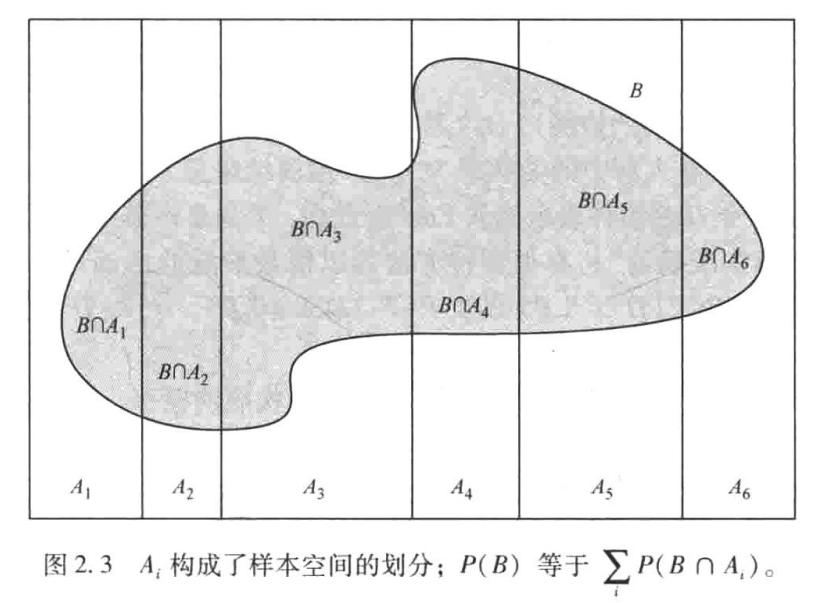
\includegraphics[width=7.5cm]{figures/全概率公式.png}
    \end{figure}

\end{frame}
\begin{frame}
  \frametitle{全概率公式( 续)}
  对于全概率公式, 我们要注意以下几点
  \begin{itemize}[<+-|alert@+>]
  \item 全概率公式的最简单形式: 如果$0<P(A)<1$, 则
    \begin{eqnarray*}
      P(B)=P(A)P(B|A)+P(\overline{A})P(B|\overline{A})
    \end{eqnarray*}
  \item 条件$A_1,A_2,\cdots,A_n$为样本空间$\Omega$的一个分割, 可改为$A_1,A_2,\cdots,A_n$互不相容, 且$B\subset \cup_{k=1}^nA_k$
  \item 在必要时,可把分割的概念推广到可列个事件($n=\infty$)的情形, 相应地有\pause
  $$ P(B)=\sum_{k=1}^{\infty} P(A_kB)=\sum_{k=1}^{\infty} P(A_k) P(B|A_k).$$
  \end{itemize}
\end{frame}



\subsection{贝叶斯公式}
\begin{frame}
	\frametitle{贝叶斯公式}
	\begin{thm}
		设$A_1,A_2,\cdots,A_n$为样本空间$\Omega$的一个分割, 即 $A_1,A_2,\cdots,A_n$互不相容, 且$\cup_{k=1}^nA_k=\Omega$, 若 $$P(B)>0, P(A_k)>0, k=1,2,\cdots,n$$ 则
		\begin{eqnarray*}
			P(A_k|B)=\dfrac{P(A_k)P(B|A_k)}{\sum_{j=1}^nP(A_j)P(B|A_j)}.
		\end{eqnarray*}
	特别的, 我们有
  \begin{eqnarray*}
    P(A|B)=\frac{P(B|A)P(A)}{P(B)}
    \end{eqnarray*}
	\end{thm}
\end{frame}


\begin{frame}{贝叶斯几率}
    \begin{defi}(\tc{几率}) 一个事件的几率(odds)为
    \begin{eqnarray*}
     ​\text{odds}(A)=P(A)/P(\overline{A})=\frac{P(A)}{1-P(A)}
     \end{eqnarray*}
    \end{defi}
  %\vspace{-0.5cm}
  \pause
  %\begin{itemize}[<+-|alert@+>]
  %\item
  \textcolor{cyan}{概率的几率表示:} $P(A)=\text{odds}(A)/(1+\text{odds(A)}) $
  %\end{itemize}
  \begin{thm} (\tc{贝叶斯公式的几率形式})对于任意两个正概率事件$A$和$B$, 给定以$B$为条件的情况下, $A$的几率如下:
   \begin{eqnarray*}
    \frac{P(A|B)}{P(\overline{A}| B)}=\frac{P(B| A)P(A)}{P(B| \overline{A})P(\overline{A})}
    \end{eqnarray*}
    \end{thm}
  \pause

  \begin{itemize}[<+-|alert@+>]
  \item 后验几率 $\dfrac{P(A|B)}{P(\overline{A}|B)}$ 等于先验几率 $\dfrac{P(A)}{P(\overline{A})}$ 乘以似然比因子 $\dfrac{P(B|A)}{P(B|\overline{A})}$. % 这个因子就是统计学中很有名的似然比.
  \item 有时候用上述形式的贝叶斯准则可以更方便地求出后验几率, 如果需要的话还可以将几率形式转换成概率形式形式.
  \end{itemize}


\end{frame}




\begin{frame}{全概率与贝叶斯内涵:由因到果,由果推因}
	\begin{itemize}[<+-|alert@+>]
		\item 在现实中把事件$B$看作结果, 把事件$A_1,A_2,\cdots, A_n$看作导致结果$B$的各种原因
		\item 全概率公式是由各种原因推理出结果事件发生的概率,是由因到果
		\item 在日常生活中常常是观察到某种现象,反推造成这种现象的各种原因的概率,即由果推因
		\item 条件概率$P(A_k|B)$, 就是在观察到结果事件$B$已经发生的情况下,推断结果事件$B$是由原因$A_k$造成的概率的大小
		\item $P(A_k)$: 先验概率, 在没有别的前提信息情况下的概率值,一般借助经验来估计,或赋予所有原因以相同的先验概率
		\item $P(A_k|B)$:后验概率, 在获得“结果事件$B$发生”这个信息之后原因$A_k$出现的概率
		\item 后验概率可看作先验概率在获取了新信息之后的一种修正, 贝叶斯公式恰恰提供了一种计算后验概率的工具

%		\item 条件概率$P(A_k|B)$通常由贝叶斯公式来计算%Bayes 公式虽然很简单, 但是它却很有哲理意义
%	%	事件原因的事前可能性估计(先验概率$P(A_k)$)$\Rightarrow$得知结果后对可能性作出新的认识(后验概率$P(A_k|B)$)
%		\item Bayes
%		\item Bayes 学派: 对概率统计问题有自己的独特理解, 但他们主张按照同等无知原则, 赋予所有原因以相同的先验概率, 常受批评
%		\item 后来有人为了取其之长避其之短, 发展出所谓经验 Bayes 方法
%		\item 在计算机广为普及的今天, Bayes 方法和经验 Bayes 方法的实用价值也随之大大提高
		\item 贝叶斯理论对于人工智能、深度学习等理论具有重要的指导意义, 贝叶斯统计受到了从未有过的青睐, 迎来了前所未有的发展机遇
	\end{itemize}
\end{frame}

\begin{frame}
  \frametitle{条件全概率公式和条件贝叶斯公式}
  \vspace{0.2cm}
    \begin{thm} (\tc{条件全概率公式}) 令$A_1,\cdots,A_n$为样本空间$\Omega$的一个划分. 设对于所有的$i$满足$P(A_iE)>0$, 则
   \begin{eqnarray*}
    P(B| E)=\sum_{i=1}^{n}P(B| A_{i},E)P(A_{i}| E)
    \end{eqnarray*}
    \end{thm}
    \pause
  \vspace{0.3cm}
  \begin{thm} (\tc{条件贝叶斯公式}) 设$P(AE)>0$且$P(BE)>0$,则有
   \begin{eqnarray*}
    P(A| B,E)=\frac{P(B| A,E)P(A| E)}{P(B| E)}
    \end{eqnarray*}
    \end{thm}

\end{frame}









\subsection{条件概率、全概率与贝叶斯公式的应用}
\begin{frame}{条件性思维谬误:控方证人的错误}
\begin{exam}\tc{(控方证人的错误)} 1988 年,Sally Clark 由于她的两个孩子在出生不久便死亡,因而被指控谋杀幼童。在审讯期间,控方的一个专家证人证实
\begin{itemize}[<+-|alert@+>]
\item 新生儿因婴儿猝死综合症 (SIDS) 而死亡的概率为 $1/8500$
\item 所以两个新生儿由于婴儿猝死综合症死亡的概率为 $(1/8500)^2$, 大约为 7300 万分之一
\item 因此,他认为 Clark 清白的概率仅为 7300 万分之一.
\end{itemize}
\end{exam}
\vspace{0.2cm}

\pause
\begin{jieda} 这个推理过程至少有两个问题
\begin{itemize}[<+-|alert@+>]
\item 一个家庭内部成员之间死于 SIDS 是否相互独立?
\begin{itemize}[<+-|alert@+>]
\item 家庭内部成员之间死于 SIDS 相互独立时,“第一个孩子死于 SIDS” 且 “第二个孩子也死于 SIDS” 的概率是相应的两个事件概率相乘
\item 如果遗传因素或其他家庭特有的风险因素导致某些家庭内的所有新生儿面临 SIDS 的风险增加,这种独立性就不再成立了.
\end{itemize}
\end{itemize}
\end{jieda}
\end{frame}

\begin{frame}{条件性思维谬误:控方证人的错误}
\begin{itemize}[<+-|alert@+>]
\item 这个所谓的专家将两个不同的条件概率混淆了: $P (\mbox{清白 | 证据})$ 和 $P (\mbox{证据 | 清白})$ 是不一样的.
\begin{itemize}[<+-|alert@+>]
\item  专家 1 声称:如果在被告人是清白的情况下,两个孩子死亡的概率很低;那就是说 $P (\mbox{证据 | 清白})$ 非常小.
\item 但人们感兴趣的是,给定现在所有的证据 (孩子均死) 条件下,报告人仍清白的概率,即 $P (\mbox{清白 | 证据})$.
\item 由贝叶斯准则可知,$$P (\mbox{清白 | 证据})=\frac{P (\mbox{证据 | 清白}) P (\mbox{清白})}{P (\mbox{证据})},$$

\item 所以为了计算 $P (\mbox{清白 | 证据})$, 这里需要考虑 $P (\mbox{清白})$, 也就是被告清白的先验概率。这个概率是很高的;
\item 虽然 SIDS 造成两个婴儿死亡是很罕见的,但是蓄意杀害两个婴儿的情况也很少见!
\item 基于现有证据的后验概率是对很低的 $P (\mbox{证据 | 清白})$ 和很高的 $P (\mbox{清白})$ 的一个平衡。专家的结果 $(1/8500)^2$ 是有问题的,它只是整个计算式中的一部分.
\end{itemize}
\end{itemize}
\end{frame}

\begin{frame}{{\rm Monty Hall}三门问题}
	\begin{exam}在 Monty Hall 主持的“Let's Make a Deal”节目中, 有三扇门, 其中有两扇门后面是一只山羊, 一扇门后面是一辆车.  选手将获得其所选中的那扇门后面的物品.
	  \begin{itemize}[<+-|alert@+>]
	  \item 一位选手从三扇最近的门中选一扇
	  \item Monty 知道车在哪扇门后面, 并以不暴露车的位置打开剩下两扇门中的一扇, 即他打开的门后面永远是山羊.
	  \item 若剩下的两扇门后都是山羊的话, Monty 会等可能地随机选一扇门.
	  \item 然后 Monty 会让对手选择, 是换另一扇没打开的门还是不换.
	  \item 如果对手的目标是得到车, 她应该换吗?
	  \end{itemize}

	  \end{exam}
	  \vspace{-0.2cm}
	   \begin{figure}[Monty Hall 问题.png]
		\centering
		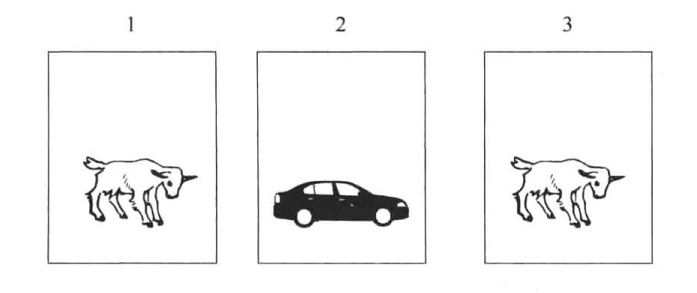
\includegraphics[width=8.5cm]{figures/Monty Hall 问题.png}
	  \end{figure}
  \end{frame}

  \begin{frame}{Monty Hall 问题(续)}
  \begin{jieda}
  \begin{itemize}[<+-|alert@+>]
  \item 先将三扇门从$1$到$3$编号. \\
  \item 不失一般性, 可以假设选手选择的是$1$号门
  \item 令
  \begin{align*}
	  A&=\{\mbox{换门得到车} \} \\
	  B&=\{\mbox{不换门得到车} \}\\
	 C_i&:=\{\mbox{车在第}i \mbox{扇门后面} \}, i=1,2,3.
  \end{align*}
  \item 显然, $P(B)=P( \mbox{不换门得到车} )=1/3$

  \item 则由全概率公式
  \begin{align*}
	  P(A)&=P(A|C_1)\cdot\frac{1}{3}+P(A|C_2)\cdot\frac{1}{3}+P(A|C_3)\cdot\frac{1}{3}\\
	 & =0\cdot\frac{1}{3}+1\cdot\frac{1}{3}+1\cdot\frac{1}{3}=\frac{2}{3}
  \end{align*}

  \end{itemize}
  \end{jieda}
  \end{frame}

  \begin{frame}{Monty Hall 三门问题图示}
	  \begin{figure}[ch1-montyhall-visual-prob.png]
		  \centering
		  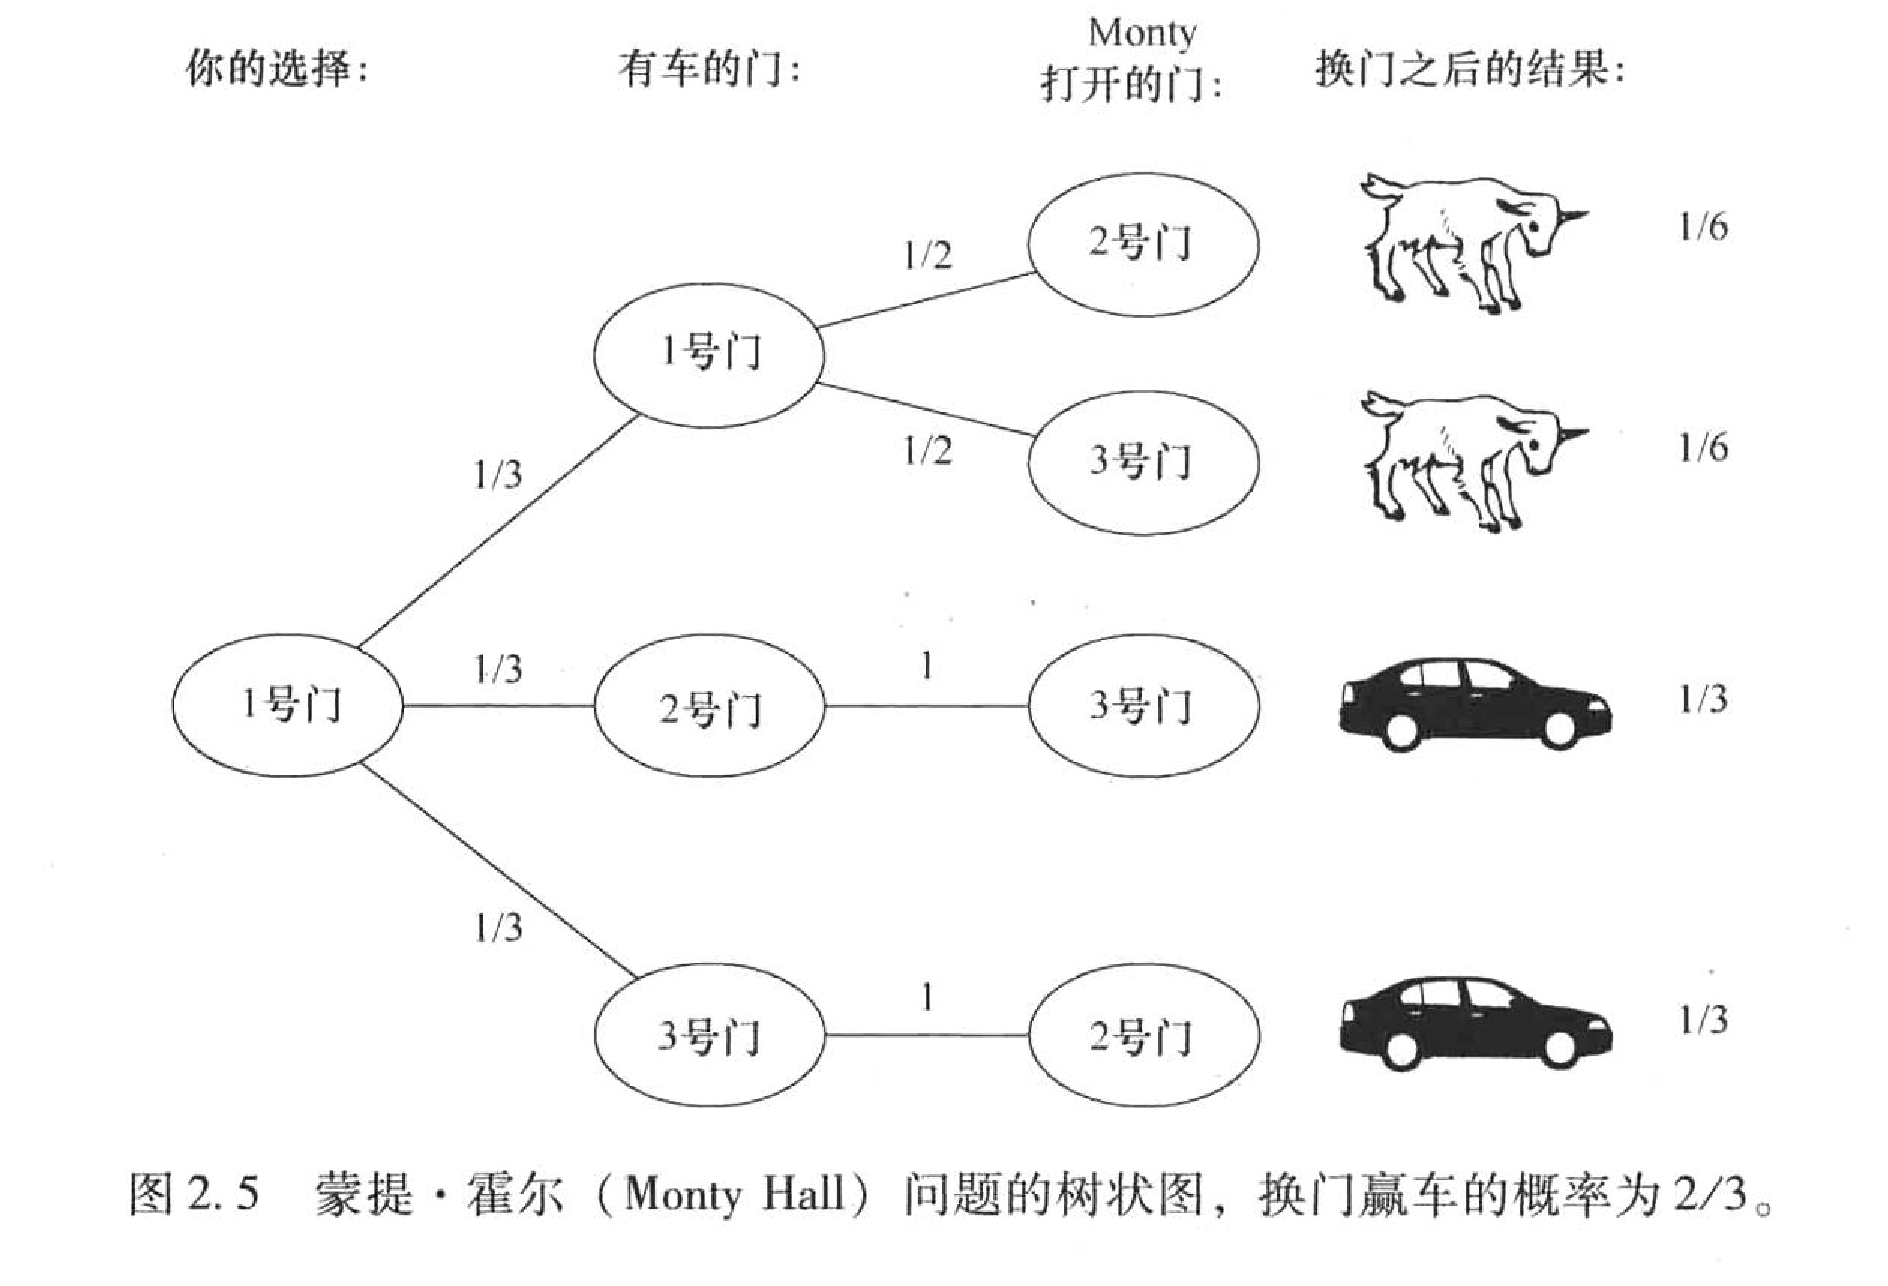
\includegraphics[width=11cm]{figures/ch1-montyhall-visual-prob.png}
		\end{figure}

  \end{frame}


  \begin{frame}{随机徘徊的吸收概率}
	\begin{exam}
		质点在数轴上整数点运动, 若质点处在整数点$i$上, 则下一时刻%
		\begin{itemize}[<+-|alert@+>]
			\item  以概率$p$向右移动到$i+1$
			\item 以概率$q$向左移动到$i-1$, 其中$p,q>0, p+q=1$
			\item 我们把质点的上述运动称之为随机徘徊或随机游动
			%\item 特殊的点$0$与$a(a>1)$
			\item 考虑数轴上的两个\textcolor{cyan}{吸收壁$0$与$a(a>1)$}:质点运动到$0$或$a$之后就永远不再移动
			\item 现求自$i(0<i<a)$出发的质点将被$0$或$a$吸收的概率
		\end{itemize}
	\end{exam}
\end{frame}


\begin{frame}
	\vspace{0.5cm}
	\hspace{-0.2cm}\jieda 令 $E_i=\{\mbox{质点自}i\mbox{出发}\}, F=\{\mbox{质点在}0\mbox{被吸收}\}, G=\{\mbox{质点在}a\mbox{被吸收}\}$. \pause

	下面对$i=0,1,\cdots,a$ 计算
	\begin{eqnarray*}
		P_i=P(F|E_i), \quad Q_i=P(G|E_i)
	\end{eqnarray*}
	\pause 记$B=\{\mbox{质点第一次向左移动 1 单位}\}$并以第 1 次可能的运动情
	况为条件进行全概率展开可得
	\begin{eqnarray*}
		Q_i&=&P(GB|E_i)+P(G\bar{B}|E_i)\\
		&=&P(B|E_i)P(G|BE_i)+P(\bar{B}|E_i)P(G|\bar{B}E_i)\\
		&=&pQ_{i+1}+qQ_{i-1}, \quad i=1,2,\cdots a-1.
	\end{eqnarray*}
	\pause 将上述递推式重写为
	\begin{eqnarray}\label{eq:ditui1}
		Q_{i+1}-Q_i=\dfrac{q}{p}(Q_i-Q_{i-1}), \quad i=1,\cdots, a-1.
	\end{eqnarray}

\end{frame}

\begin{frame}
	\vspace{0.5cm}
	\begin{enumerate}[<+-|alert@+>]
		\item 当$p=q=1/2$时, 由$Q_0=0$及$Q_a=1$可得
		\begin{eqnarray*}
			Q_i=\dfrac{i}{a},\quad  i=0,\cdots, a.
		\end{eqnarray*}
		\item 当$p\neq q$时, 反复利用递推式\eqref{eq:ditui1}并注意到$Q_0=0$可导出
		\begin{eqnarray}\label{eq:ditui2}
			Q_{i+1}-Q_i=\bigg(\dfrac{q}{p}\bigg)^iQ_1, \quad i=1,\cdots, a-1.
		\end{eqnarray}
		\pause 上式对$i=1,\cdots, a-1$求和并利用$Q_a=1$可得
		\begin{eqnarray*}
			Q_1=\bigg[\sum_{i=0}^{a-1}\bigg(\dfrac{q}{p}\bigg)^{i}\bigg]^{-1}=\dfrac{1-q/p}{1-(q/p)^a}
		\end{eqnarray*}
		\pause 再将(\ref{eq:ditui2})式对$i=1,\cdots, i-1$求和并将上述$Q_1$代入可得
		\begin{eqnarray*}
			Q_i=\dfrac{1-(q/p)^i}{1-(q/p)^a}, \quad i=0,\cdots, a.
		\end{eqnarray*}

	\end{enumerate}
\end{frame}

\begin{frame}
	综上可得
	\begin{eqnarray*}
		Q_i=\left\{
		\begin{array}{cl}
			\dfrac{i}{a}, &p=q,\\
			\\
			\dfrac{1-(q/p)^i}{1-(q/p)^a}, &p\neq q.
		\end{array}
		\right.
	\end{eqnarray*}
	类似可得



	\begin{eqnarray*}
		P_i=\left\{
		\begin{array}{cl}
			\dfrac{a-i}{a}, &p=q,\\
			\\
			\dfrac{(q/p)^i-(q/p)^a}{1-(q/p)^a}, &p\neq q.
		\end{array}
		\right.
	\end{eqnarray*}


\end{frame}



\begin{frame}{Simpson 悖论}
	\begin{exam}
		有两种治疗肾结石的方案,其治疗效果如下:
		\begin{itemize}[<+-|alert@+>]
			\item \textcolor{cyan}{方案$1$:} 小结石患者占$25\%$, 大结石患者占$75\%$, 小结石患者的治愈率是$93\%$, 大结石患者的治愈率是$73\%$
			\item \textcolor{cyan}{方案$2$:} 小结石患者占$77\%$, 大结石患者占$23\%$, 小结石患者的治愈率是$87\%$, 大结石患者的治愈率是$69\%$
			\item 不管是对小结石患者, 还是大结石患者, 方案$1$的治愈率都要高于方案$2$
			\item \textcolor{red}{方案$1$优于方案$2$吗?}
		\end{itemize}
	\end{exam}
	\pause
	\begin{jieda}
		计算两种方案的治愈率
		\begin{itemize}[<+-|alert@+>]
			\item 记$A$=\{患者是小结石患者\}, $B$=\{患者被治愈\}
			\item 根据全概率公式\pause
			\begin{align*}
				&\hspace{-0.5cm}P_1(B)=\pause P_1(A)P_1(B|A)+P_1(\overline{A})P_1(B|\overline{A})=\pause 0.25·0.93+0.75·0.73=0.78\pause \\
				&\hspace{-0.5cm} P_2(B)=\pause P_2(A)P_2(B|A)+P_2(\overline{A})P_2(B|\overline{A})=\pause 0.77·0.87+0.23·0.69=0.8286
			\end{align*}
			\item 方案$2$的治愈率高于方案$1$, 可见方案$1$并不优于方案$2$
		\end{itemize}
	\end{jieda}
\end{frame}

\begin{frame}
	\frametitle{敏感性问题调查}
	敏感性问题调查方案的关键在于要使被调查者愿意作出真实的回答又能保守个人秘密, 如果调查方案有误, 被调查者就会拒绝配合, 所得调查数据将失去真实性.
	\pause
	\vspace{0.5cm}

	{\bf 调查方案: } 被调查者只需要加答以下两个问题中的一个问题,且只需要回答“是”或“否”.

	\pause
	问题 A: 你的生日是否在 7 月 1 日之前?

	问题 B: 所调查的敏感性问题.

	\pause
	\vspace{0.5cm}
	{\bf 调查方案的操作: }

	( 1)被调查者在没有旁人的情况下独自一人在房间内操作回答问题

	\pause
	( 2)被调查者从一个罐子中随机抽一球, 看过颜色后放回, 若抽到白球, 回答问题 A, 抽到红球, 回答问题 B.

	( 3)被调查者无论回答问题 A 还是问题 B, 只需在仅有“是”与“否”选项的答卷上作答然后将答卷放入密封的投票箱内.

\end{frame}

\begin{frame}
	\frametitle{敏感性问题调查}
	{\bf \textcolor{red}{问题:}} 假若我们有$n$张问卷, 其中$k$张回答“是”, 我们如何确定选定红球回答问题 B 为“是”的概率?


	\pause
	{\bf \textcolor{red}{已知:}}
	\begin{itemize}[<+-|alert@+>]
		\item 红白球的比例, 即$P(\mbox{红球}):=\pi, P(\mbox{白球})=1-\pi$;
		\item $P(\mbox{是}|\mbox{白球})=0.5$;
		\item $P(\mbox{是})\approx \dfrac{k}{n}$.
	\end{itemize}
	\pause
	{\bf \textcolor{red}{待求:}} $p:=P(\mbox{是}|\mbox{红球})$.

	\pause
	{\bf\jieda} 由全概率公式可得
	\begin{eqnarray*}
		P(\mbox{是})=P(\mbox{白球})P(\mbox{是}|\mbox{白球})+P(\mbox{红球})P(\mbox{是}|\mbox{红球})
	\end{eqnarray*}
	即\pause
	\begin{eqnarray*}
		\dfrac{k}{n}\approx (1-\pi)\cdot 0.5+\pi\cdot p \Rightarrow p=\dfrac{k/n-0.5(1-\pi)}{\pi}
	\end{eqnarray*}


\end{frame}

\begin{frame}{{\rm Bayesian}滤波}
\begin{itemize}[<+-|alert@+>]
	\item 许多工程科学类问题都可以归结为如下图所示形式
	\begin{figure}[htbp]\nonumber
		\centering
		\includegraphics<+->[width=9.19cm, height=3cm]{BayesianFilter.jpg}
		% \caption{}
  %\onslide<4->\centering{\small 心灵捕手 }
	  \end{figure}
	\item  系统自身的状态 \( X \) 是我们关注的随机事件,但是由于技术手段等方面的限制,无法直接对 \( X \) 进行观测, 只能获取另一随机事件, 即间接反映系统状态 \( X \) 的观测量 \( Z \).
	\item 问题转化为已知观测量 \( Z \) 的条件下, 如何对系统状态 \( X \) 进行推断.用条件概率的语言讲, 就是计算 \( P(X \mid Z) \).
	\item 通常情况下, \( X \) 和 \( Z \) 随时间变化,分别记作 \( X_{n} \) 和 \( Z_{n} \) ,其中 \( n \) 表示时间. 那么在实际应用中, 到 \( n \) 时刻为止, 我们掌握的实际观测数据为 \( \left\{Z_{1}, \cdots, Z_{n}\right\} \),
\end{itemize}


\end{frame}


\begin{frame}{{\rm Bayesian}滤波}
\begin{itemize}[<+-|alert@+>]
	\item 如何实现 $P\left(X_{n} | Z_{1}, \cdots, Z_{n}\right) \longrightarrow P\left(X_{n+1} | Z_{1}, \cdots, Z_{n+1}\right)$的递推计算?
	\item 注意到, 若已知$X_{n+1}$时,$Z_{n+1}$与$\left\{Z_{1}, \cdots, Z_{n}\right\}$独立, 则
	{\small\begin{eqnarray*}
		P\left(X_{n+1} | Z_{1}, \cdots, Z_{n+1}\right)&=&  \pause\frac{P\left(X_{n+1}, Z_{1}, \cdots, Z_{n+1}\right)}{P\left(Z_{1}, \cdots, Z_{n+1}\right)}\\
		&=& \pause\frac{P\left(Z_{n+1} | X_{n+1}, Z_{1}, \cdots, Z_{n}\right) P\left(X_{n+1}, Z_{1}, \cdots, Z_{n}\right)}{P\left(Z_{1}, \cdots, Z_{n+1}\right)}\\
		&=&\pause \frac{P\left(Z_{n+1} | X_{n+1}\right) P\left(X_{n+1}, Z_{1}, \cdots, Z_{n}\right)}{P(Z_{n+1}|Z_{1}, \cdots, Z_n)P\left(Z_{1}, \cdots, Z_{n+1}\right)}
	\end{eqnarray*}}




\end{itemize}



\end{frame}

\begin{frame}{{\rm Bayesian}滤波}
	\begin{itemize}[<+-|alert@+>]
		\item 再由\pause
		{\small \begin{eqnarray*}
			&&P\left(X_{n+1}, Z_{1}, \cdots, Z_{n}\right)\\
			&=&\pause\sum_{X_{n}} P\left(X_{n+1}, X_{n}, Z_{1}, \cdots, Z_{n}\right) \\
			&=&\pause\sum_{X_{n}} P\left(X_{n+1} | X_{n}, Z_{1}, \cdots, Z_{n}\right) P\left(X_{n} | Z_{1}, \cdots, Z_{n}\right) P\left(Z_{1}, \cdots, Z_{n}\right) \\
			&=&\pause\sum_{X_{n}} P\left(X_{n+1} | X_{n}\right) P\left(X_{n} | Z_{1}, \cdots, Z_{n}\right) P\left(Z_{1}, \cdots, Z_{n}\right)\pause
		\end{eqnarray*}}
	    \item 将上式代入前面一页表达式中可得
	{\small \[
		\hspace{-0.3cm} P\left(X_{n+1} | Z_{1}, \cdots, Z_{n+1}\right)\pause=\frac{P\left(Z_{n+1} | X_{n+1}\right)}{P\left(Z_{n+1} | Z_{n}, \cdots, Z_{1}\right)} \sum_{X_{n}} P\left(X_{n+1} | X_{n}\right) P\left(X_{n} | Z_{1}, \cdots, Z_{n}\right)\]}
		\item 上式便是对系统状态进行递推估计的 Bayesian 滤波公式,在雷达、声呐、通信、导航、机器学习等许多领域有广泛应用.

	\end{itemize}






	\end{frame}
%%% Local Variables:
%%% mode: latex
%%% TeX-master: t
%%% End:
